%!TEX root = ../DigSig2.tex
\section{FIR Digital Filter Design\buch{Chapter 10}}

\subsection{Window Method\buchSeite{532-541}}
\subsubsection{Ideal Filters\buchSeite{532-534}}
Ideal frequency responses (Fig. \ref{fig:freqresp}) are transformed into infinite impulse responses $d(k)$ (eq: \ref{eq:impresp}), which are then made finite using a particular window.

\begin{figure}[htp]
\begin{subfigure}{0.49\textwidth}
\centering
\newcommand{\coordinates}{coordinates {
(-3.14,1) (-1.569,1) (-1.571,0)
( 1.571,0) (1.569,1) ( 3.14,1)
};}
\begin{tikzpicture}[
trim axis left,
trim axis right
]
\begin{axis}[
	every axis plot post/.append style={mark=none},
	width=0.5\textwidth, height=0.25\textwidth,
	scale only axis,
	xmin=-3.14, xmax=3.14,
	ymin=0, ymax=1.2,
	xlabel=$\omega$,
	ylabel=$D(\omega)$,
	axis x line=bottom, axis y line=middle, enlargelimits=upper,
	xtick={-3.14,-1.57,0,1.57, 3.14}, xticklabels={$-\pi$, $-\omega_c$, 0, $\omega_c$, $\pi$}
	]
	\expandafter\addplot\coordinates
\end{axis}
\end{tikzpicture}
\caption{Highpass}
\end{subfigure}
\begin{subfigure}{0.49\textwidth}
\centering
\newcommand{\coordinates}{coordinates {(-3.14,0) (-1.569,0) (-1.571,1) (1.571,1) (1.569,0) (3.14,0)};}
\begin{tikzpicture}[
trim axis left,
trim axis right
]
\begin{axis}[
	every axis plot post/.append style={mark=none},
	width=0.5\textwidth, height=0.25\textwidth,
	scale only axis,
	xmin=-3.14, xmax=3.14,
	ymin=0, ymax=1.2,
	xlabel=$\omega$,
	ylabel=$D(\omega)$,
	axis x line=bottom, axis y line=middle, enlargelimits=upper,
	xtick={-3.14,-1.57,0,1.57, 3.14}, xticklabels={$-\pi$, $-\omega_c$, 0, $\omega_c$, $\pi$}
	]
	\expandafter\addplot\coordinates
\end{axis}
\end{tikzpicture}
\caption{Lowpass}
\end{subfigure}

\begin{subfigure}{0.49\textwidth}
\centering
\newcommand{\coordinates}{coordinates {
(-3.14,1) (-2.001,1) (-1.999,0) (-1.001,0) (-0.999,1)
(0.999,1) ( 1.001,0) ( 1.999,0) ( 2.001,1) ( 3.14,1)};}
\begin{tikzpicture}[
trim axis left,
trim axis right
]
\begin{axis}[
	every axis plot post/.append style={mark=none},
	width=0.5\textwidth, height=0.25\textwidth,
	scale only axis,
	xmin=-3.14, xmax=3.14,
	ymin=0, ymax=1.2,
	xlabel=$\omega$,
	ylabel=$D(\omega)$,
	axis x line=bottom, axis y line=middle, enlargelimits=upper,
	xtick={-3.14,-2, -1,0,1,2, 3.14}, xticklabels={$-\pi$, $-\omega_b$, $-\omega_a$, 0, $\omega_a$, $\omega_b$, $\pi$}
	]
	\expandafter\addplot\coordinates
\end{axis}
\end{tikzpicture}
\caption{Bandstop}
\end{subfigure}
\begin{subfigure}{0.49\textwidth}
\centering
\newcommand{\coordinates}{coordinates {
(-3.14,0) (-2.001,0) (-1.999,1) (-1.001,1) (-0.999,0)
(0.999,0) (1.001,1) (1.999,1) (2.001,0) ( 3.14,0)};}
\begin{tikzpicture}[
trim axis left,
trim axis right
]
\begin{axis}[
	every axis plot post/.append style={mark=none},
	width=0.5\textwidth, height=0.25\textwidth,
	scale only axis,
	xmin=-3.14, xmax=3.14,
	ymin=0, ymax=1.2,
	xlabel=$\omega$,
	ylabel=$D(\omega)$,
	axis x line=bottom, axis y line=middle, enlargelimits=upper,
	xtick={-3.14,-2, -1,0,1,2, 3.14}, xticklabels={$-\pi$, $-\omega_b$, $-\omega_a$, 0, $\omega_a$, $\omega_b$, $\pi$}
	]
	\expandafter\addplot\coordinates
\end{axis}
\end{tikzpicture}
\caption{Bandpass}
\end{subfigure}

\begin{subfigure}{0.49\textwidth}
\centering
\newcommand{\coordinates}{coordinates {(-3.14,-1) (3.14,1)};}
\begin{tikzpicture}[
trim axis left,
trim axis right
]
\begin{axis}[
	every axis plot post/.append style={mark=none},
	width=0.5\textwidth, height=0.25\textwidth,
	scale only axis,
	xmin=-3.14, xmax=3.14,
	xlabel=$\omega$,
	ylabel=$D(\omega)/j$,
	axis x line=middle, axis y line=middle, enlargelimits=upper,
	xtick={-3.14,0,3.14}, xticklabels={$-\pi$,  0, $\pi$}
	]
	\expandafter\addplot\coordinates
\end{axis}
\end{tikzpicture}
\caption{Differentiator}
\end{subfigure}
\begin{subfigure}{0.49\textwidth}
\centering
\newcommand{\coordinates}{coordinates {(-3.14,1) (-0.001,1) (0.001,-1) (3.14,-1) };}
\begin{tikzpicture}[
trim axis left,
trim axis right
]
\begin{axis}[
	every axis plot post/.append style={mark=none},
	width=0.5\textwidth, height=0.25\textwidth,
	scale only axis,
	xmin=-3.14, xmax=3.14,
	xlabel=$\omega$,
	ylabel=$D(\omega)/j$,
	axis x line=middle, axis y line=middle, enlargelimits=upper,
	xtick={-3.14,0,3.14}, xticklabels={$-\pi$,  0, $\pi$}
	]
	\expandafter\addplot\coordinates
\end{axis}
\end{tikzpicture}
\caption{Hilbert transformer}
\end{subfigure}

\caption{Ideal frequency responses\buchSeite{533}}
\label{fig:freqresp}
\end{figure}


\begin{equation}
d(k) = \int_{-\pi}^{\pi}D(\omega) e^{j\omega k}\frac{d\omega}{2\pi} \label{eq:impresp}
\end{equation}

\begin{align*}
&\text{lowpass filter} && d(k) = \frac{\sin(\omega_ck)}{\pi k} \\
&\text{highpass filter} && d(k) = \delta(k) - \frac{\sin(\omega_ck)}{\pi k} \\
&\text{bandpass filter} && d(k) = \frac{\sin(\omega_bk) - \sin(\omega_ak)}{\pi k} \\
&\text{bandstop filter} && d(k) = \delta(k) - \frac{\sin(\omega_bk) - \sin(\omega_ak)}{\pi k} \\
&\text{differentiator} && d(k) = \frac{\cos(\pi k)}{k}-\frac{\sin(\pi k)}{\pi k^2}\\
&\text{Hilbert transformer} && d(k) = \frac{1-\cos(\pi k)}{\pi k}
\end{align*}

Note that the highpass / lowpass filters and the bandpass / bandstop
filters are complementary:
\begin{align*}
	d_{LP}(k) + d_{HP}(k) &= \delta(k) \qquad \Leftrightarrow \qquad D_{LP}(\omega) + D_{HP}(\omega) = 1 \\
	d_{BP}(k) + d_{BS}(k) &= \delta(k) \qquad \Leftrightarrow \qquad D_{BP}(\omega) + D_{BS}(\omega) = 1
\end{align*}

The frequency responses of the differentiator and the Hilbert transformers
are both imaginary and odd, while the other frequency responses are real
and even. The impulse responses of the differentiator and the Hilbert
transformer are therefore real and odd.

\subsubsection{Window comparison}
\begin{tabular}{|l|c|c|c|c|c|c|}
	\hline
	Window & $\delta$ & $A_{stop}$ & $A_{pass}$ & $D$ & $R$ & $c$ \\
	\hline
	Rectangular & 8.9\% & $-21$ dB & $1.55$ dB & 0.92 & $-13$ dB & 1\\
	Hamming & 0.2\% & $-54$ dB & $0.03$ dB & 3.21 & $-40$ dB & 2\\
	Kaiser & variable $\delta$ & $-20\log_{10}\delta$ & $17.372\delta$ & $D = \left\{
						\begin{array}{l l}
							\frac{A-7.95}{14.36}& \quad \text{if } A>21\\
							0.922 & \quad \text{if } A \leq 21
						\end{array} \right.$ & variable R & $6(R+12)/55$\\
	\hline
\end{tabular}

\subsubsection{Rectangular Window\buchSeite{535}}
\begin{multicols}{2}
	\begin{itemize}
		\item Simplest window, Length $N = 2M+1$
		\item truncate the infinite impulse response: \\ $-M \leq k \leq M$
		\item $\rightarrow \mathbf{d} = [d_{-M}, ..., d_{-1}, d_0, d_1, ..., d_M]$
		\item The resulting causal FIR Filter must be delayed by M samples \newline
		$\rightarrow \mathbf{h} = \mathbf{d} = [h_0, h_{M-1}, h_M, h_{M+1}, ..., h_{2M}]$
	\end{itemize}

	\begin{center}
		\begin{tikzpicture}
\begin{axis}[axis lines=left,width=8cm,height=4cm,xmin=-3,xmax=3,ymin=0,ymax=3]
\addplot+[ycomb] coordinates{
		(-2,1)
		(-1,2)
		(0,3)
		(1,2)
		(2,1)

	};
\end{axis}

\node at (1,-0.9) {$-M$};
\node at (5.5,-0.9) {$+M$};

\draw[decorate,decoration=brace,yshift=-0.2cm] (5.5,-1.0) -- node[below=0.3cm] {$N$} (1,-1.0);


\end{tikzpicture}
	\end{center}
\end{multicols}

\subsubsection{Hamming Window\buchSeite{540}}
\begin{itemize}
	\item Improved passband and stopband ripple suppression at the cost of a wider transition width.
	\item Hamming window impulse response:
	\begin{align*}
		w(n) = 0.54 -0.46\cos\left(\frac{2\pi n}{N-1}\right),&&n= 0,1,\dots,N-1
	\end{align*}
	\item Filter impuls response:
	\begin{align*}
		h(n) = w(n)d(n-M),&&-\infty < n < \infty
	\end{align*}
	\item e.g. lowpass filter
	\begin{align*}
		h(n) = \left[0.54 -0.46\cos\left(\frac{2\pi n}{N-1}\right)\right]\cdot\frac{\sin(\omega_c(n-M))}{\pi (n-M)}
	\end{align*}
\end{itemize}

\newpage
\subsubsection{Kaiser Window\buchSeite{541}}
The Kaiser window is a window family, where the overshoot and the steepness
are controlled by two parameters. \\

\begin{center}
	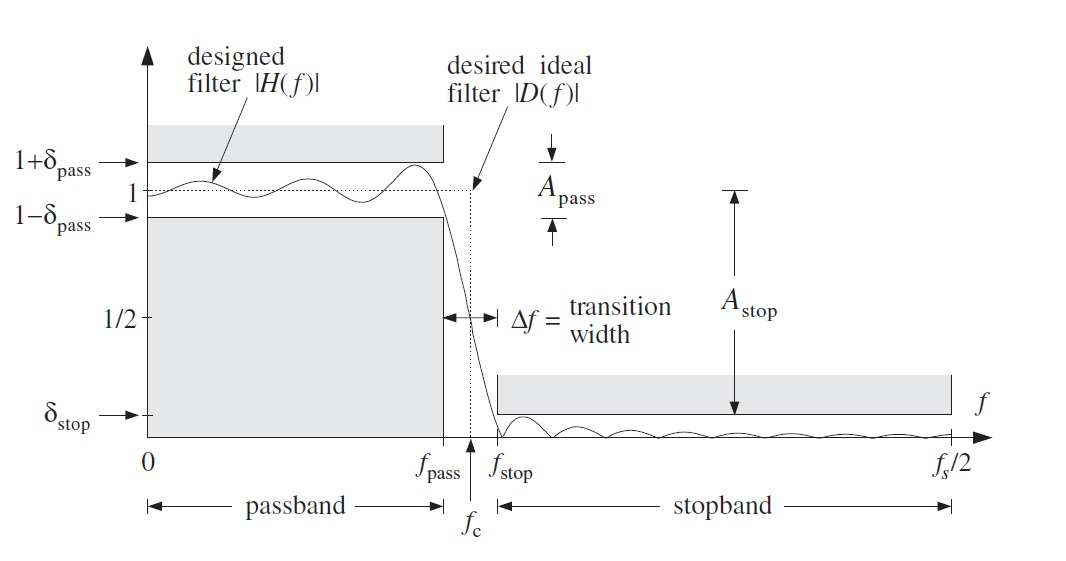
\includegraphics[width=10cm]{images/FIR_KaiserSpecs.jpg}
\end{center}

\begin{tabular}{|l|l|}
	\hline
	cutoff frequency & $f_c=\frac{1}{2}(f_{pass}+f_{stop})$ \\ \hline
	transition width & $\Delta f = f_{stop}-f_{pass}$\\ \hline
	passband/stopband frequency & $f_{pass} = f_c - \frac{1}{2}\Delta f,\quad f_{stop}= fc+\frac{1}{2}\Delta f$\\ \hline
	digital frequencies & $\omega_{pass}=\frac{2\pi f_{pass}}{f_s},\quad \omega_{stop}=\frac{2\pi f_{stop}}{f_s},\quad
						  \omega_{c}=\frac{2\pi f_c}{f_s},\quad \Delta\omega=\frac{2\pi \Delta f}{f_s}$\\ \hline
	passband/stopband overshoot & $A_{pass}=20\log_{10}\left(\frac{1+\delta_{pass}}{1-\delta_{pass}}\right),\quad A_{stop}=-20\log_{10}\delta_{stop}$\\
								& $\delta_{pass}=\frac{10^{A_{pass}/20}-1}{10^{A_{pass}/20}+1},\quad \delta_{stop} = 10^{-A_{stop}/20}$ \\ \hline
	window parameters &
		$\alpha = \left\{
					\begin{array}{l l}
						0.1102(A-8.7)& \quad \text{if } A \geq 50\\
						0.5842(A-21)^{0.4}+0.07886(A-21) & \quad \text{if }21 < A < 50\\
						0 & \quad \text{if } A \leq 21
					\end{array} \right. $\\
	&	$D = \left\{
					\begin{array}{l l}
						\frac{A-7.95}{14.36}& \quad \text{if } A>21\\
						0.922 & \quad \text{if } A \leq 21
					\end{array} \right. $\\ \hline
	window function & $w(n)=\frac{I_0(\alpha\sqrt{1-(n-M)^2/M^2})}{I_0(\alpha)}=\frac{I_0(\alpha\sqrt{n(2M-n)}/M)}{I_0(\alpha)},$ \\
	& $I_0=\text{modified Bessel function of the first kind and 0th order.}$\\
	\hline
\end{tabular}

\paragraph{Design steps for a lowpass filter with Kaiser Window\buchSeite{544}}
\begin{enumerate}
\item Calculate $f_c$, $\Delta f$ and $\omega_c$.
\item Calculate $\delta_{pass}$ and $\delta_{stop}$.
\item Calculate $\delta=\min(\delta_{pass},\delta_{stop})$ and $A=-20log_{10}\delta$ in dB. \newline
	  The filter will have equal passband and stopband ripples. Therefore the design must be based on the smaller of the two ripples.
\item Calculate $\alpha$ and $D$.
\item Calculate the filter length $N=\frac{Df_s}{\Delta f}+1$ and round it up to the next \textbf{odd} number. Calculate $M=(N-1)/2$.
\item Calculate the window function $w(n),\quad n=0,1,\dots,N-1$
\item Calculate the windowed impuls response $h(n)=w(n)d(n-M)$.
\end{enumerate}

\subsubsection{Rules for different filter types}
\paragraph{Highpass filter}~\\
The role of $f_{pass}$ and $f_{stop}$ are interchanged, therefore $\Delta f = f_{pass}-f_{stop}$

\paragraph{Bandpass filter}~\\
\begin{center}
	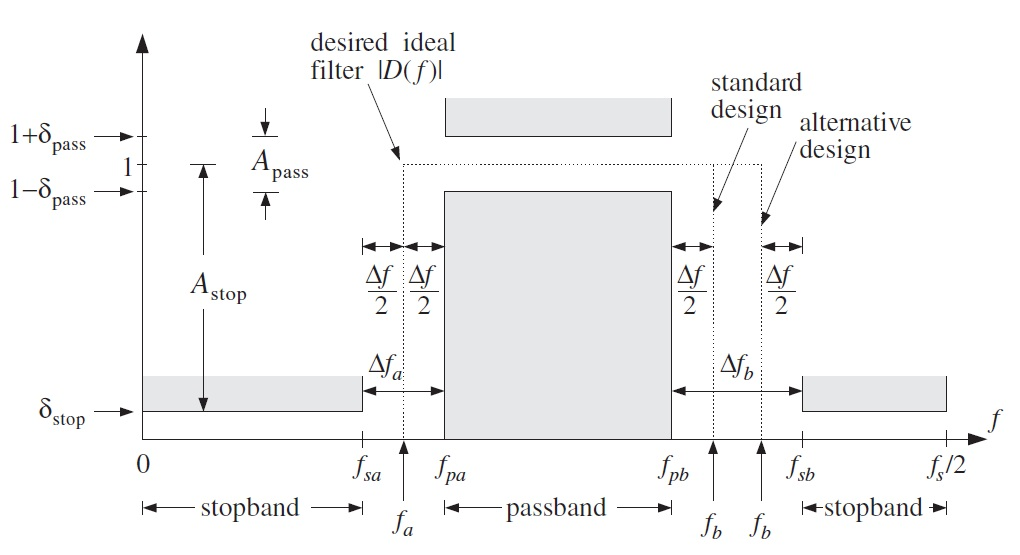
\includegraphics[width=8cm]{images/FIR_KaiserBP.jpg}
\end{center}
The final filter design will have equal transition widths, therefore
$\Delta f = \min(\Delta f_a, \Delta f_b)$ with $\Delta f_a=f_{pa}-f_{sa}$
and $\Delta f_b=f_{sb}-f_{pb}$.
Since the transition widths are different, one can select $f_a$ and $f_b$ either
with focus on the passband (standard), or with focus on the stop band:
\begin{align*}
	f_a &= f_{pa} - \frac{1}{2} \Delta f \:, \qquad f_b = f_{pb} + \frac{1}{2} \Delta f \qquad \text{focus on pass band}\\
	f_a &= f_{sa} + \frac{1}{2} \Delta f \:, \qquad f_b = f_{sb} - \frac{1}{2} \Delta f \qquad \text{focus on stop band}
\end{align*}

\subsubsection{Kaiser Window for Spectral Analysis\buchSeite{555}}
The Kaiser window can of course be used for spectral analysis (DFT, FFT). As it
has a variable shape, the factor $c$ can be varied. For a given side lobe level
$R$, the factor $c$ can be calculated as
\begin{equation*}
	c = \frac{6 \left(R + 12\right)}{155}
\end{equation*}
The shape parameter $\alpha$ of the Kaiser window is calculated by
\begin{equation*}
	\alpha = \begin{cases}
		0\:, & R < 13.26 \\
		0.76609(R-13.26)^{0.4}+0.09834(R-13.26)\:, & 13.26 < R < 60 \\
		0.12438 (R+6.3)\:, & 60 < R < 120
	\end{cases}
\end{equation*}

\subsection{Frequency Sampling Method\buchSeite{558}}
For an arbitrary frequency response $D(\omega)$, the inverse DTFT cannot
be given by the integral
$d(k) = \int_{-\pi}^{\pi}D(\omega) e^{j\omega k}\frac{d\omega}{2\pi}$
from equ. \ref{eq:impresp}. Therefore this integral is approximated by the
following sum
\begin{equation*}
	\tilde{d}(k) = \frac{1}{N} \sum\limits_{i=-M}^M D(\omega_i) e^{j \omega_i k} \:, \qquad -M \leq k \leq M
\end{equation*}

If $N = 2M+1$, then this is basically an inverse $N$-point DFT with discrete
frequencies from $-\pi \ldots \pi$. Any length-$N$ window discussed in this
section can be used to create a delayed and windowed version of $\tilde{d}$:
\begin{equation*}
	h(n) = w(n) \tilde{d}(n-M) \:, \qquad n = 0,1,\ldots,N-1
\end{equation*}

\subsection{Other FIR Design Methods\buchSeite{558}}
Though the Kaiser window is simple and flexible, sometimes there are methods
which are better suited. The Parks-McClellan method is based on the so-called
\emph{equiripple Chebyshev approximation}, which often leads to smaller filters.
The main difference is that the ripples do not decrease, but always stay the
same height.
